% ****** Start of file apssamp.tex ******
%
%   This file is part of the APS files in the REVTeX 4.1 distribution.
%   Version 4.1r of REVTeX, August 2010
%
%   Copyright (c) 2009, 2010 The American Physical Society.
%
%   See the REVTeX 4 README file for restrictions and more information.
%
% TeX'ing this file requires that you have AMS-LaTeX 2.0 installed
% as well as the rest of the prerequisites for REVTeX 4.1
%
% See the REVTeX 4 README file
% It also requires running BibTeX. The commands are as follows:
%
%  1)  latex apssamp.tex
%  2)  bibtex apssamp
%  3)  latex apssamp.tex
%  4)  latex apssamp.tex
%
\documentclass[%
 reprint,
%superscriptaddress,
%groupedaddress,
%unsortedaddress,
%runinaddress,
%frontmatterverbose, 
%preprint,
%showpacs,preprintnumbers,
%nofootinbib,
%nobibnotes,
%bibnotes,
 amsmath,amssymb,
 aps,
%pra,
%prb,
%rmp,
%prstab,
%prstper,
%floatfix,
]{revtex4-1}

\usepackage{graphicx}% Include figure files
\usepackage{dcolumn}% Align table columns on decimal point
\usepackage{bm}% bold math
%\usepackage{hyperref}% add hypertext capabilities
%\usepackage[mathlines]{lineno}% Enable numbering of text and display math
%\linenumbers\relax % Commence numbering lines

%\usepackage[showframe,%Uncomment any one of the following lines to test 
%%scale=0.7, marginratio={1:1, 2:3}, ignoreall,% default settings
%%text={7in,10in},centering,
%%margin=1.5in,
%%total={6.5in,8.75in}, top=1.2in, left=0.9in, includefoot,
%%height=10in,a5paper,hmargin={3cm,0.8in},
%]{geometry}

%custom commands
% $Id: commands.tex 909 2013-06-03 14:10:59Z rpreghen $
% Adaptation of a file originally by Roberto Preghenella (thanks!) 

\newcommand{\Om}{$\Omega^-$}
\newcommand{\Mo}{$\overline{\Omega}^+$}
\newcommand{\X}{$\Xi^-$}
\newcommand{\Ix}{$\overline{\Xi}^+$}
\newcommand{\Xis}{$\Xi^{\pm}$}
\newcommand{\Oms}{$\Omega^{\pm}$}
\newcommand{\meanpt}{$\langle p_\mathrm{t}\rangle$}
\newcommand{\nineH}{$\sqrt{s}~=~0.9$~TeV}
\newcommand{\seven}{$\sqrt{s}~=~7$~TeV}
\newcommand{\twoH}{$\sqrt{s}~=~0.2$~TeV}
\newcommand{\dndy}{d$N$/d$y$}
\newcommand{\LT}{L{\'e}vy-Tsallis}
\newcommand{\GeVc}{GeV/$c$}
\newcommand{\MeVc}{MeV/$c$}
\newcommand{\GeVcs}{GeV/$c$ }
\newcommand{\MeVcs}{MeV/$c$ }
\newcommand{\GeVmass}{GeV/$c^2$}
\newcommand{\MeVmass}{MeV/$c^2$}
\newcommand{\allpart}{\kzero, \lmb, \almb, \X, \Ix, \Om and \Mo}

\newcommand{\ITS}          {\rm{ITS }}
\newcommand{\TOF}          {\rm{TOF }}
\newcommand{\ZDC}          {\rm{ZDC }}
\newcommand{\ZDCs}         {\rm{ZDCs }}
\newcommand{\ZNA}          {\rm{ZNA }}
\newcommand{\ZNC}          {\rm{ZNC }}
\newcommand{\SPD}          {\rm{SPD }}
\newcommand{\SDD}          {\rm{SDD }}
\newcommand{\SSD}          {\rm{SSD }}
\newcommand{\TPC}          {\rm{TPC }}
\newcommand{\VZERO}        {\rm{VZERO }}
\newcommand{\VZEROA}       {\rm{VZERO-A }}
\newcommand{\VZEROC}       {\rm{VZERO-C }}
\newcommand{\pip}          {\ensuremath{\pi^{+}}}
\newcommand{\pim}          {\ensuremath{\pi^{-}}}
\newcommand{\pipm}          {\ensuremath{\pi^{\pm}}}
\newcommand{\kap}          {\ensuremath{\mathrm{K}^{+}}}
\newcommand{\kam}          {\ensuremath{\mathrm{K}^{-}}}
\newcommand{\kapm}          {\ensuremath{\mathrm{K}^{\pm}}}
\newcommand{\p}               {$\rm p$}
\newcommand{\pbar}         {$\rm\overline{p}$}
\newcommand{\kzero}        {\ensuremath{{\rm K}^{0}_{S}}}
\newcommand{\kstar}        {\ensuremath{{\rm K}^{*0}}}
\newcommand{\lmb}          {\ensuremath{\Lambda}}
\newcommand{\almb}         {\ensuremath{\overline{\Lambda}}}
%this is another analysis...
%\newcommand{\allpart}      {$\pi^{\pm}$, K$^{\pm}$, \kzero, p(\pbar) and \lmb(\almb)}
\newcommand{\degree}       {$^{\rm o}$}
\newcommand{\dg}           {\mbox{$^\circ$}}
\newcommand{\dedx}         {\ensuremath{\mathrm{d}E/\mathrm{d}x}}
\newcommand{\pp}           {pp}
\newcommand{\ppbar}        {\mbox{$\mathrm {p\overline{p}}$}}
\newcommand{\PbPb}         {\mbox{Pb--Pb}}
\newcommand{\pPb}          {\mbox{p--Pb}}
\newcommand{\AuAu}         {\mbox{Au--Au}}
\newcommand{\pseudorap}    {\mbox{$\left | \eta \right | $}}
\newcommand{\dNdeta}       {\ensuremath{\mathrm{d}N_\mathrm{ch}/\mathrm{d}\eta}}

\newcommand{\avdNdeta}       {\ensuremath{\left<\mathrm{d}N_\mathrm{ch}/\mathrm{d}\eta\right>}}
\newcommand{\dNchdy}         {\ensuremath{\mathrm{d}N_\mathrm{ch}/\mathrm{d}y}}
\newcommand{\dNdy}         {\ensuremath{\mathrm{d}N/\mathrm{d}y} }
\newcommand{\dNdyst}       {\ensuremath{\sqrt{\frac{dN_\pi/dy}{s_T}}}}
\newcommand{\dNdetatr}     {\mathrm{d}N_\mathrm{tracklets}/\mathrm{d}\eta}
\newcommand{\dNdetar}[1]   {\mathrm{d}N_\mathrm{ch}/\mathrm{d}\eta\left.\right|_{|\eta|<#1}}
\newcommand{\lum}          {\, \mbox{${\rm cm}^{-2} {\rm s}^{-1}$}}
\newcommand{\barn}         {\, \mbox{${\rm barn}$}}
\newcommand{\m}            {\, \mbox{${\rm m}$}}
\newcommand{\ncls}         {\ensuremath{N_{cls}}}
\newcommand{\nsigma}       {\ensuremath{n\sigma}}
\newcommand{\dcaxy}        {\ensuremath{{\rm DCA}_{xy}} }
\newcommand{\dcaz}         {\ensuremath{{\rm DCA}_{z}} }
\newcommand{\EcrossB}      {E$\times$B}%{\ensuremath{{\rm E}\times{\rm B}}}
\newcommand{\bb}           {Bethe-Bloch}
\newcommand{\s}            {\ensuremath{\sqrt{s}}}
\newcommand{\pt}           {\ensuremath{p_{\rm T}}}
\newcommand{\pts}           {\ensuremath{p_{\rm T}} }
\newcommand{\hlab}         {\ensuremath{\eta_{\rm lab}}}
\newcommand{\ynn}         {\ensuremath{y_{\rm NN}}}
\newcommand{\ycms}         {\ensuremath{y_{\rm CMS}}}
\newcommand{\ylab}         {\ensuremath{y_{\rm lab}}}
\newcommand{\ppi}          {\ensuremath{{\rm p}/\pi}}
\newcommand{\kpi}          {\ensuremath{{\rm K}/\pi}}
\newcommand{\lpi}          {\ensuremath{{\rm \Lambda}/\pi}}
%\newcommand{\ppi}          {\ensuremath{(\pi^+ + \pi^-)/({\rm K}^+ + {\rm K}^-)}}
%\newcommand{\kpi}          {\ensuremath{({\rm p} + {\rm \bar p})/({\rm K}^+ + {\rm K}^-)}}
\newcommand{\mt}           {\ensuremath{m_{\rm T}}}
\newcommand{\snn}          {\ensuremath{\sqrt{s_{\rm NN}}}}
\newcommand{\snnbf}        {\ensuremath{\mathbf{{\sqrt{s_{\mathbf NN}}}}}}
\newcommand{\sonly}        {\ensuremath{\sqrt{s}}}
\newcommand{\Npart}        {\ensuremath{N_\mathrm{part}}}
\newcommand{\avNpart}      {\ensuremath{\langle N_\mathrm{part} \rangle}}
\newcommand{\avNpartdata}  {\ensuremath{\langle N_\mathrm{part}^{\rm data} \rangle}}
\newcommand{\Ncoll}        {\ensuremath{N_\mathrm{coll}}}
\newcommand{\Dnpart}       {\ensuremath{D\left(\Npart\right)}}
\newcommand{\DnpartExp}    {\ensuremath{D_{\rm exp}\left(\Npart\right)}}
\newcommand{\dNdetapt}     {\ensuremath{\dNdeta\,/\left(0.5\Npart\right)}}
\newcommand{\dNdetaptr}[1] {\ensuremath{\dNdetar{#1}\,/\left(0.5\Npart\right)}}
\newcommand{\dNdetape}     {\left(\ensuremath{\dNdeta\right)/\left(\avNpart/2\right)}}
\newcommand{\dNdetaper}[1] {\ensuremath{\dNdetar{#1}\,/\left(\avNpart/2\right)}}
\newcommand{\dndydpt}      {\ensuremath{{\rm d}^2N/({\rm d}y {\rm d}p_{\rm t})}}
\newcommand{\abs}[1]       {\ensuremath{\left|#1\right|}}
\newcommand{\signn}        {\ensuremath{\sigma^{\rm inel.}_{\rm NN}}}
\newcommand{\vz}           {\ensuremath{V_{z}}}
\newcommand{\Tfo}          {\ensuremath{{T}_{\rm kin}}}
\newcommand{\Tch}          {\ensuremath{{T}_{\rm ch}}}
\newcommand{\bT}           {\ensuremath{\beta_{\rm T}}}
\newcommand{\avbT}         {\ensuremath{\left< \beta_{\rm T}\right>}}
\newcommand{\avpT}         {\ensuremath{\left< \pt \right>}\xspace}
\newcommand{\muB}          {\ensuremath{\mu_{B}}}
\newcommand{\stat}         {({\it stat.})}
\newcommand{\syst}         {({\it sys.})}
\newcommand{\Fig}[1]       {Fig.~\ref{#1}}
\newcommand{\Figure}[1]    {Figure~\ref{#1}}
\newcommand{\Ref}[1]       {Ref.~\cite{#1}}
\newcommand{\green}[1]     {\textcolor{green}{#1}}
\newcommand{\blue}[1]      {\textcolor{blue}{#1}}
\newcommand{\red}[1]       {\textcolor{red}{#1}}
\newcommand{\white}[1]     {\textcolor{white}{#1}}
\newcommand{\gevc}         {\ensuremath{{\rm GeV}/c}}
\newcommand{\mevc}         {\ensuremath{{\rm MeV}/c}}
\newcommand{\gevcs}         {\ensuremath{{\rm GeV}/c} }
\newcommand{\mevcs}         {\ensuremath{{\rm MeV}/c} }
\newcommand{\avg}[1]       {\ensuremath{\left\langle#1\right\rangle}}

\newcommand {\dEdx}      {d\textit{E}/d\textit{x}\xspace}
\newcommand {\Zvtx}   {\ensuremath{Z_\mathrm{vtx}}\xspace}
\newcommand {\pT}   {\pt}

\newcommand {\proton}     		{\ensuremath{p}}
\newcommand {\electron}   		{\Pe}
\newcommand {\pion}    	  		{\ensuremath{\pi}}
\newcommand {\kaon}       		{\ensuremath{K}}
\newcommand {\KTopi}      		{\kaon/\pion}
\newcommand {\pTopi}      		{\proton/\pion}
\newcommand {\KzeroShort} 		{\PKzS}
\newcommand {\lambdaBaryon} 	{\PGL}
\newcommand {\antiLambdaBaryon} {\PAGL}
\newcommand {\gammaPhoton} 		{\PGg}
\newcommand {\Nevt}      {\ensuremath{N_\mathrm{evt}}\xspace}
\newcommand {\NevtMB}  {\ensuremath{N_\mathrm{evt|MB}}\xspace}
\newcommand {\NevtMBVTX}  {\ensuremath{N_\mathrm{evt|(MB\, \&\, Vtx)}}\xspace}
\newcommand {\NevtMBVTXZ}  {\ensuremath{N_\mathrm{evt|(MB\, \& Vtx\, \&\, \textit{Z}_{vtx})}}\xspace}
\newcommand {\NevtINEL}  {\ensuremath{N_\mathrm{evt}(\textsc{inel})}\xspace}
\newcommand {\fPrim}       {\ensuremath{f_{\mathrm{prim}}}\xspace}
\newcommand {\NPrim}     {\ensuremath{N_{\mathrm{prim}}}\xspace}
\newcommand {\NSec}      {\ensuremath{N_{\mathrm{sec}}}\xspace}
\newcommand {\NPrimTilde}     {\ensuremath{\widetilde{N}_{\mathrm{prim}}}\xspace}
\newcommand {\NSecTilde}      {\ensuremath{\widetilde{N}_{\mathrm{sec}}}\xspace}
\newcommand {\NTilde}      {\ensuremath{\widetilde{N}}\xspace}

\newcommand{\pPiplus}{\ensuremath{{\pi}^{+}}\xspace}
\newcommand{\pPiminus}{\ensuremath{{\pi}^{-}}\xspace}
\newcommand{\sPi}{\ensuremath{{\pi}}\xspace}
\newcommand{\pKplus}{\ensuremath{{\rm K}^{+}}\xspace}
\newcommand{\pKminus}{\ensuremath{{\rm K}^{-}}\xspace}
\newcommand{\sProton}{\ensuremath{\rm p}\xspace}
\newcommand{\pProton}{\ensuremath{\rm p}\xspace}
\newcommand{\apProton}{\ensuremath{\overline{\rm p}}\xspace}
\newcommand{\sPr}{\ensuremath{\rm p}\xspace}
\newcommand{\sKzero}{\ensuremath{2{\rm K}^{0}_{S}}\xspace}
\newcommand{\pKzero}{\ensuremath{{\rm K}^{0}_{S}}\xspace}
\newcommand{\sLambda}{\ensuremath{\Lambda}\xspace}
\newcommand{\pLambda}{\ensuremath{\Lambda}\xspace}

\newcommand{\LtoKzero}{\ensuremath{\Lambda}/\ensuremath{{\rm K}^{0}_{S}}\xspace}
\newcommand{\apLambda}{\ensuremath{\overline{\Lambda}}\xspace}
\newcommand{\sXi}{\ensuremath{\Xi}\xspace}
\newcommand{\pXi}{\ensuremath{\Xi^{-}}\xspace}
\newcommand{\apXi}{\ensuremath{\overline{\Xi}^{+}}\xspace}
\newcommand{\sOmega}{\ensuremath{\Omega}\xspace}
\newcommand{\pOmega}{\ensuremath{\Omega^{-}}\xspace}
\newcommand{\apOmega}{\ensuremath{\overline{\Omega}^{+}}\xspace}

\newcommand{\betaT}{\ensuremath{\langle \beta_{T}\rangle}\xspace}
\newcommand{\Tkin}{\ensuremath{T_{kin}}\xspace}

\renewcommand{\labelitemi} {$-$}
%==========================================================%
%%% inline warnings for internal discussion 
%\newcommand{\warn}[1]      {\textbf{\textcolor{red}{[#1]}}}
\newcommand{\warn}[1]      {{\small\textbf{\textcolor{red}{(!\footnote{\textbf{(!)}~#1})}}}}
%\newcommand{\warn}[1]      {{\small\textbf{(!\footnote{\textbf{(!)}~#1})}}\marginpar{\textbf{---}}}
\newcommand{\todo}[1]      {\textbf{\textcolor{red}{[TODO: #1]}}}
%%% fake numbers
\newcommand{\fake}[1]      {\textbf{\textcolor{red}{#1}}}
%\newcommand{\fake}[1]      {#1}
\newcommand{\final}[1]     {\textbf{\textcolor{blue}{#1}}}
\newcommand{\prelim}[1]    {\textbf{\textcolor{magenta}{#1}}}
\renewcommand{\mod}[1]       {\textbf{\textcolor{red}{#1}}}


%document
\begin{document}

\preprint{APS/123-QED}

\title{Testing coalescence and statistical-thermal production scenarios\\for (anti-)(hyper-)nuclei and exotic QCD objects at LHC energies}
%\thanks{A footnote to the article title}%

\author{Francesca Bellini}
\email{francesca.bellini@cern.ch}
\author{Alexander P. Kalweit}%
\email{alexander.kalweit@cern.ch}
\affiliation{European Organization for Nuclear Research (CERN) \\Geneva, Switzerland}

\date{\today}% It is always \today, today,
             %  but any date may be explicitly specified

\begin{abstract}

We present a detailed comparison of coalescence and thermal-statistical models for the production of (anti-)(hyper-)nuclei in high-energy collisions. For the first time, such a study is carried out as a function of the size of the object relative to the size of the particle emitting source. Our study reveals large differences between the two scenarios for the production of objects with extended wave-functions. While both models give similar predictions and show similar agreement with experimental data for (anti-)deuterons and (anti-)\hethree\ nuclei, they largely differ in their description of (anti-)hyper-triton production.
We propose to address experimentally the comparison of the production models by measuring the coalescence parameter systematically for different (anti-)(hyper-)nuclei in different collision systems and differentially in multiplicity. 
Such measurements are feasible with the current and upgraded LHC experiments. 
Our findings highlight the unique potential of ultra-relativistic heavy-ion collisions as a laboratory to clarify the internal structure of exotic QCD objects and can serve as a basis for more refined calculations in the future.

%\begin{description}
%\item[Usage]
%Secondary publications and information retrieval purposes.
%\item[PACS numbers]
%May be entered using the \verb+\pacs{#1}+ command.
%\item[Structure]
%You may use the \texttt{description} environment to structure your abstract;
%use the optional argument of the \verb+\item+ command to give the category of each item. 
%\end{description}
\end{abstract}

\pacs{Valid PACS appear here}% PACS, the Physics and Astronomy
                             % Classification Scheme.
\keywords{(Anti-)nuclei, hyper-triton, coalescence, thermal model}%Use showkeys class option if keyword
                              %display desired
\maketitle

\section{Introduction} 
Nuclei and hyper-nuclei are special objects with respect to non-composite hadrons (pions, protons, etc.), because their size is comparable to a fraction or the whole system created in high-energy proton-proton (pp), proton-nucleus (pA) and nucleus-nucleus (AA) collisions~\cite{Adam:2015vna}.  
Their size is typically defined as the rms of their (charge) wave-function, corresponding to about 2 fm for light (anti-)nuclei as obtained from electron scattering experiments. 
For the hyper-triton, theoretical calculations indicate a rms of the wave-function of about 5 fm \cite{Nemura:1999qp}, significantly larger than that of non-strange nuclei with mass number $A = 3$ and driven by the average separation of the $\Lambda$ with respect to the two other nucleons.
The properties of the objects under study here are summarised in Tab. \ref{tab:nucleusradii}.

\begin{table*}[htb]

\centering

\begin{ruledtabular}
\begin{tabular}{cccccccc}\\[-2ex]
Mass number & Nucleus &  Composition  & Binding energy (MeV)   &  Spin & \rmsradius$^{meas}$~(fm) &  $r_{A}$ (fm) & Refs. 
\\[0.5ex] \hline \\[-2ex]
      A = 2                     & d                                    & pn                                  &   2.224575 (9)     &     1   & 2.1413 $\pm$ 0.0025      &  3.2    &   \cite{VanDerLeun:1982bhg,Mohr:2015ccw}     \\[0.5ex]  \hline \\[-2ex]
      A = 3  & \tritium 	                  & pnn                               &    8.4817986 (20) & 1/2   &  1.755  $\pm$ 0.086        &  2.15   &   \cite{Purcell:2015gtm}           \\
                                   & \hethree                         & ppn                                &   7.7180428  (23) & 1/2  & 1.959 $\pm$  0.030         &   2.48  &   \cite{Purcell:2015gtm} \\
                                   & \hthreelambda               & p$\Lambda$n                &    0.13 $\pm$ 0.05 & 1/2  &  4.9 --  10.0                    &  6.8 -- 14.1 & \cite{Davis:2005mb,Nemura:1999qp} \\[0.5ex]                                    
\end{tabular}
\end{ruledtabular}

\caption{Properties of nuclei and hyper-nuclei with mass number $A \leq 3$. The nucleus size is given in terms of the (charge) rms radius of the wave-function, \rmsradius. The size parameter of the wave-function of the harmonic oscillator potential,  $r_{A}$, is chosen such that the measured/expected rms,  \rmsradius$^{meas}$~(fm), is approximately reproduced. The proton rms charge radius $\lambda_{p} = 0.879(8)$ fm \cite{bernauer10} is subtracted from $\rmsradius^{meas}$  according to $\rmsradius = \sqrt{(\rmsradius^{meas})^2 - {\lambda_{p}^2}}$ to account for the finite extension of the constituents. We assume $\lambda_{\Lambda}\approx \lambda_{n}\approx \lambda_{p}$.}
\label{tab:nucleusradii}
\end{table*}


For about sixty years, coalescence models have been used to describe the formation of composite objects \cite{Butler:1963, Kapusta:1980, Sato:1981ez, Nagle:1996vp, Scheibl:1998tk, Cho:2017dcy, Blum:2017qnn, Bazak:2018hgl, Zhao:2018lyf}.
Surprisingly, thermal-statistical models have been successful in describing also the production of light (anti-)(hyper-)nuclei across a wide range of energies in AA collisions \cite{Andronic:2010qu,Andronic:2017}. 
In this approach, particles are produced from a fireball in thermal and kinetic equilibrium with temperatures of the order of $T_{chem} \approx$ 156 MeV.
Particle abundances are fixed at chemical freeze-out, when inelastic collisions cease. Further elastic and pseudo-elastic collisions occur among the components of the expanding fireball, that can affect the spectral shapes and the measurable yields of short-lived (strongly decaying) hadronic resonances. Once the mean free path for elastic collisions is larger than the system size, the fireball freezes-out kinetically at $T_{kin} \approx$ 90 MeV~\cite{Abelev:2013vea}. 
In such a dense and hot environment, composite objects with binding energies that are small with respect to the temperature of the system, appear as ``fragile''. 
For instance, the binding energy of the deuteron is $B_{E, d}$ = 2.2 MeV $\ll T_{chem}, T_{kin}$.
The cross-section for pion-induced deuteron breakup is significantly larger than the typical (pseudo)-elastic cross-sections for the re-scattering of hadronic resonance decay products \cite{Garcilazo:1982yc, Bass:1998ca, Schukraft:2017nbn}. 
Similarly, the elastic cross-section driving deuteron spectra to kinetic equilibration in central heavy-ion collisions \cite{Acharya:2017dmc} is smaller than the breakup cross-section \cite{Garcilazo:1982yc, Bass:1998ca, Schukraft:2017nbn}.   
The deuterons produced at chemical freeze-out would be expected not to survive the hadronic phase, yet their production is measured to be consistent with statistical-thermal model predictions and a non-zero elliptic flow is observed \cite{Acharya:2017dmc}. 
Several solutions have been proposed to solve this ``light (anti-)nuclei puzzle'': (a.) a sudden freeze-out at the QGP-hadron phase boundary, (b.) the thermal production of these objects as compact quark bags \cite{Andronic:2017}, and (c.) the coincidence of coalescence and thermal production \cite{Scheibl:1998tk, HeinzTorino}. 
Data from rescattering of short-lived hadronic resonances suggest a long-lasting hadronic phase \cite{Abelev:2014uua}, thus strongly disfavouring hypothesis (a.). 
While hypothesis (b.) cannot presently be tested beyond the agreement of measured (anti-)nuclei yields with statistical-thermal model predictions, hypothesis (c.) is scrutinised in this letter.

To this purpose, we compare LHC data to models. 
For the first time, these data allow for the systematic study of the light (anti-)(hyper-)nuclei production as a function of the system- and object-size. 
A quantitative comparison of the two scenarios has been proposed in \cite{Mrowczynski:2016xqm}, resulting in the idea to study the production rates of nuclei with similar mass but very different internal structure, as \hefour~and ${}^{4}\mathrm{Li}$ \cite{Bazak:2018hgl}. However, as ${}^{4}\mathrm{Li}$ is not stable with respect to strong decay, its measurement is experimentally difficult and probably less constraining than the comparison with the hyper-nuclei proposed here.
We propose that \bA~is systematically measured in all collision systems by exploiting the large statistics sample foreseen at the LHC Run 3 \& 4, in order to discriminate the aforementioned scenarios.
 
\section{Coalescence approach} \label{sec:coalescence}

In the coalescence picture, nucleons produced in the collision coalesce into nuclei if they are close in space and have similar velocities \cite{Butler:1963,Kapusta:1980}. 
For a nucleus with mass number $A = Z + N$, the coalescence probability is quantified by the coalescence parameter $B_{A}$.
Considering that at LHC energies the number of produced protons and neutrons at midrapidity is expected to be equal,  $B_{A}$ is defined as

\begin{equation}
E_{A}\frac{\mathrm{d}^{3}N_{A}}{\mathrm{d}p_{A}^{3}}=B_{A}{\left(E_{\mathrm{p,n}}\frac{\mathrm{d}^{3}N_{\mathrm{p,n}}}{\mathrm{d}p_{\mathrm{p,n}}^{3}}\right)^{A}}\left\vert_{\vec{p}_{\mathrm{p}}=\vec{p}_{\mathrm{n}}=\frac{\vec{p}_{A}}{A}} \right..
\label{eq:BA}
\end{equation}
%
where $p_{\mathrm{p,n}}$ are the momenta of the proton and neutron and $E_{p,n}$ their energies.
%
The LHC is particularly suited for the production of anti-nuclei, since the number of baryons and anti-baryons is essentially equal at midrapidity \cite{Abbas:2013rua}. Consequently, the anti-particle to particle ratio for (hyper-)nuclei is consistent with unity \cite{ALICE:nucleipp2017, anielski-HQ14, Acharya:2017dmc, Adam:2015yta}.

In a simple coalescence approach, \bA~is expected to be independent of momentum and of the object size relative to the volume of particle emission (hereafter referred to as ``source volume'' or ``size'').
While this picture is found to be approximately valid in pp and \pPb~collisions \cite{ALICE:nucleipp2017, anielski-HQ14}, it breaks down in \PbPb~collisions, which exhibit a strong decrease of $B_{A}$ with centrality \cite{ALICE:deuteronppPbPb2015}. 
The elliptic flow of deuterons cannot be explained by simple coalescence \cite{Acharya:2017dmc}. 

More advanced coalescence models \cite{Sato:1981ez, Nagle:1996vp, Scheibl:1998tk} take into account the source size, as the coalescence probability naturally decreases for nucleons with similar momenta that are produced far apart in configuration space. We rely on the formalism proposed in~\cite{Scheibl:1998tk}.
As coalescence is a quantum-mechanical process, the classical definition of phase space is replaced by the Wigner formalism. The production probability of a nucleon cluster is given by the overlap of the Wigner function with the phase-space distributions of the constituents.
The wave-functions of the (hyper-)nuclei are approximated by the ground-state wave-functions of an isotropic spherical harmonic oscillator as in~\cite{Scheibl:1998tk} with one single characteristic-size parameter, $r_{A}$. 
For the deuteron wave-function $\varphi_{d}(\vec{r}) $, one obtains

\begin{equation}\label{eq:WaveHeinz}
 \varphi_{d}(\vec{r}) = (\pi r_{d}^2)^{-3/4} \exp\left(-{r^2 \over 2 r_{d}^2}\right) \;.
\end{equation}

\noindent For nuclei with $A > 2$, analogous forms exist. The relation between $r_{A}$ and the rms of the wave-function was derived in~\cite{Shebeko:2006ud} as

\begin{equation}
 \rmsradius^2 = {3 \over 2}{A - 1 \over A} {r_{A}^2 \over 2}
\end{equation} 

\noindent for point-like constituents. 
We follow the gaussian ansatz to obtain fully analytic solutions.
In Tab.~\ref{tab:nucleusradii}, we list the measured rms of the wave-function, $\rmsradius^{meas}$, and the $r_{A}$ parameter derived from these relations. 
We encourage future more rigorous numerical studies that address the calculation of coalescence probabilities with more realistic wave-functions, e.g. the Hulthen parameterisation for deuterons \cite{Nagle:1996vp} or a $\Lambda$-deuteron parameterisation for hyper-tritons as done only for central collisions in~\cite{Zhang:2018euf}. 

The quantum-mechanical nature of the coalescence products is explicitly accounted for by means of an average correction factor, $\langle C_{A} \rangle$. For deuterons, $\langle C_{d} \rangle$ has been approximated as 

\begin{equation}
\langle C_{d} \rangle \approx \frac{1}{\left[1+ \left(\frac{\dradius}{2R_{\perp}(m_{T})}\right)^{2}\right] \sqrt{1+ \left(\frac{\dradius}{2R_{\|}(m_{T})}\right)^{2}}}
\label{eq:Cd}
\end{equation}
%
where \dradius~is the size parameter, \rperp~and \rpar~are the lengths of homogeneity of the coalescence volume and $m_{T}$ is the transverse mass of the coalescing nucleons.
The nucleus size enters in the  calculation of \btwo~via $\langle C_{d} \rangle$, as well as the homogeneity volume $\rperp^{2}\rpar$, according to the relation~\cite{Scheibl:1998tk}
%
\begin{equation}
\btwo = \frac{3\pi^{3/2} \langle C_{d} \rangle}{2m_{T}\rperp^{2}(m_{T})\rpar(m_{T})} \;\; .
\label{eq:B2cd}
\end{equation}
%
The coalescence parameter decreases with increasing volume, as expected. 
$\langle C_{d} \rangle$ introduces a length scale defined by the deuteron size relative to the source size. 
If we assume that  $\rperp \approx \rpar \approx R$, Eqs. \ref{eq:Cd} and \ref{eq:B2cd} simplify to 

\begin{equation}
\langle C_{d} \rangle \approx \left[1+ \left(\frac{\dradius}{2R(m_{T})}\right)^{2}\right]^{-3/2}
\label{eq:Cdapprox}
\end{equation}
%
and
%
\begin{equation}
\btwo = \frac{3\pi^{3/2} \langle C_{d} \rangle}{2m_{T}R^{3}(m_{T})}.
\label{eq:B2approx}
\end{equation}
%

Figure \ref{fig:radiusDependence} shows the source radius ($R$) dependence of $\langle C_{d} \rangle$ and \btwo, calculated assuming (a.) $\dradius = 0$, (b.) $\dradius = 0.3$ fm, (c.) the actual value $\dradius = 3.2$ fm~\cite{Mohr:2015ccw}, (d.) a larger, irrealistic $\dradius = 10$ fm. 
As shown in Fig. \ref{fig:radiusDependence}, $\langle C_{d} \rangle$ suppresses significantly the production of objects with radius larger than the source. 

\begin{figure}[ht]
\begin{center}
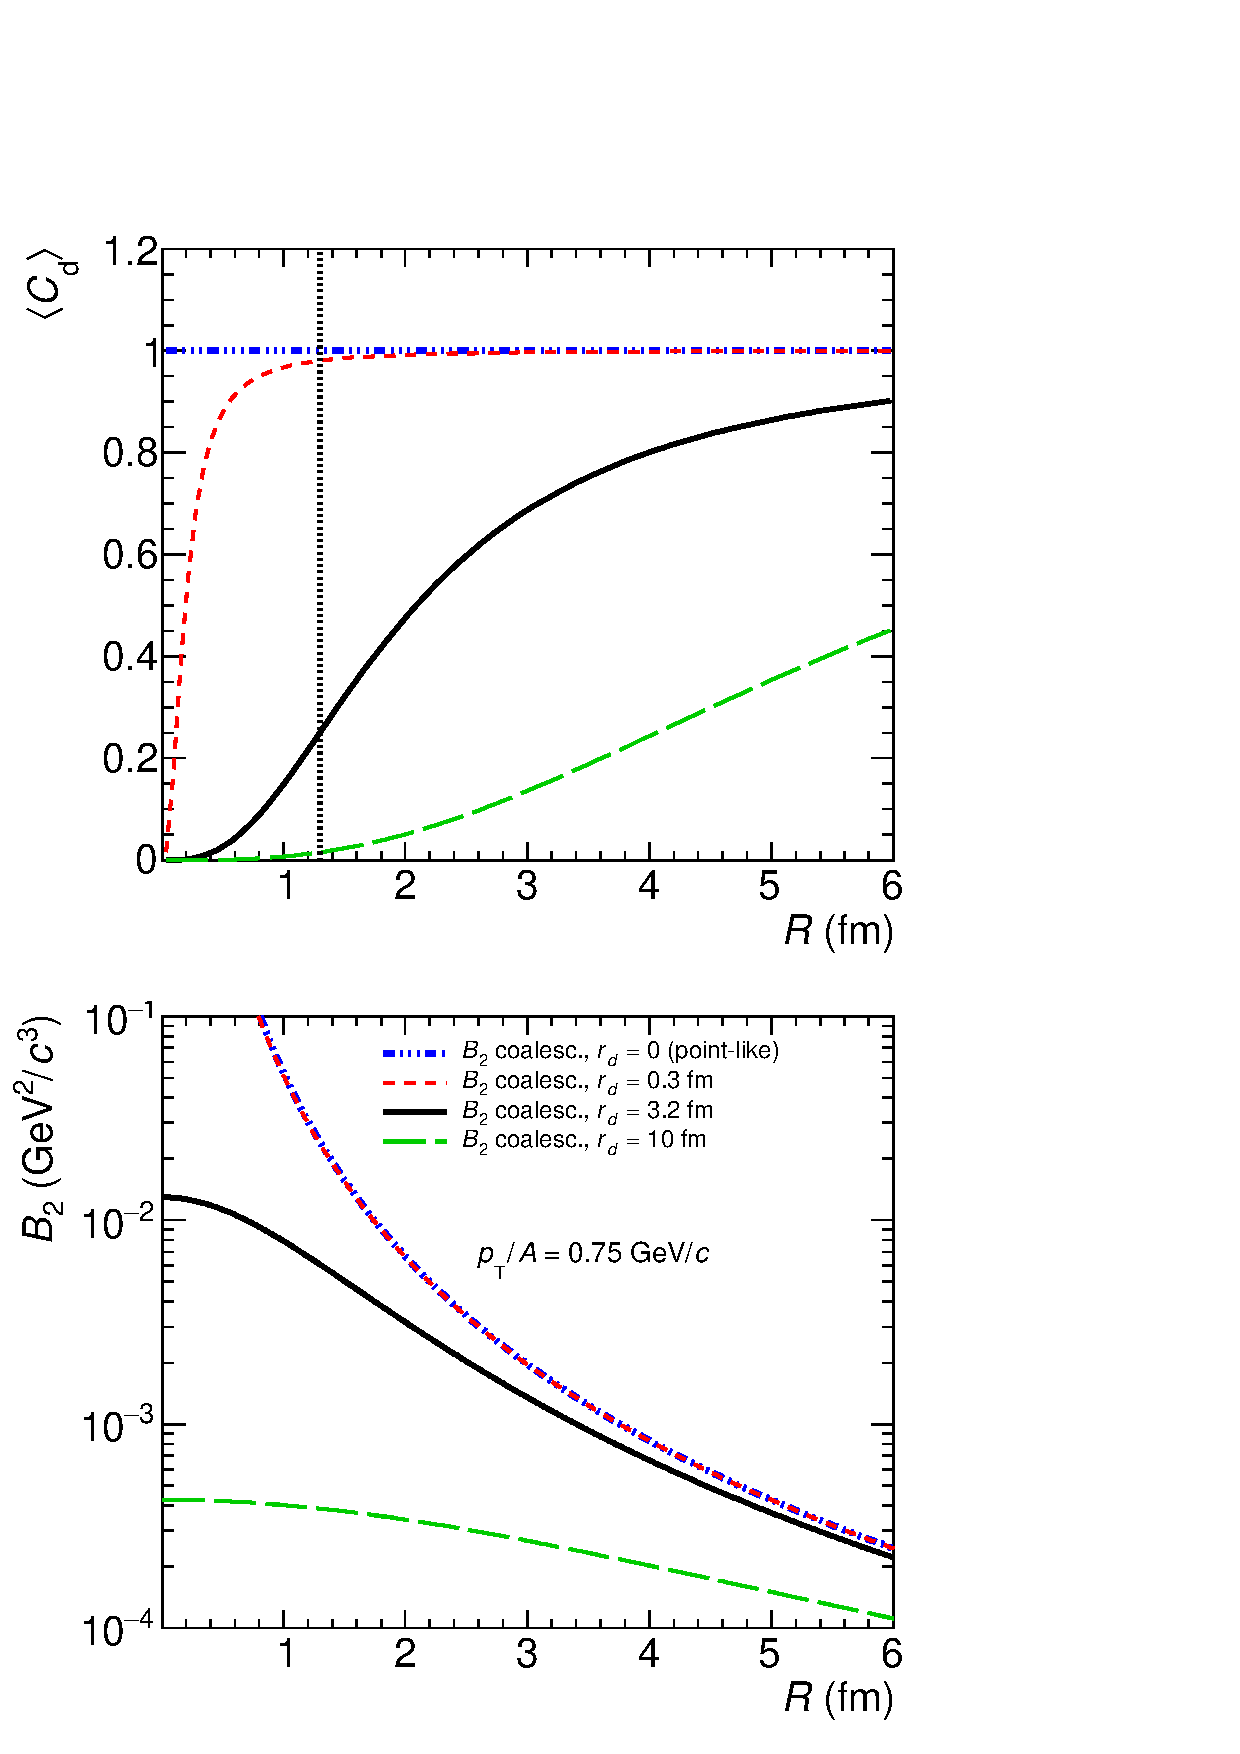
\includegraphics[width=\columnwidth]{../theory_coalescence_Cd_B2_vert.png}
\caption{{The quantum-mechanical correction factor $\langle C_{d} \rangle$ (left panel, see Eq.~\ref{eq:Cdapprox}) and the coalescence parameter \btwo~for deuteron (right panel, see Eq.~\ref{eq:B2approx}) as a function of the radius of the source $R$, calculated assuming a size parameter for the deuteron $\dradius = 0, 0.3, 3.2$ and $10$ fm. The inflection point of $\langle C_{d} \rangle$ corresponds to $R = \dradius/\sqrt{6}$ and is indicated in the left panel by the vertical dotted line for $\dradius = 3.2$ fm.}}
\label{fig:radiusDependence}
\end{center}
\end{figure}   

Following the discussion in~\cite{Blum:2017qnn}, Eq.~\ref{eq:Cd} may be generalised as 

\begin{equation}
\langle C_{A} \rangle = \prod_{i=1,2,3} \left(1 + \frac{r^2}{4R_{i}^2} \right)^{-\frac{1}{2}(A-1)} \;\; .
\label{eq:CA_general}
\end{equation}
%
Similarly, the coalescence parameter \bA~for a nucleus with mass number $A$ and spin $J_{A}$ is generalised by Eq. 6.2 of~\cite{Scheibl:1998tk}.
For the case of \hethree, the latter becomes Eq. 9 of~\cite{Blum:2017qnn}.

In summary, under the assumption $R_1\approx R_2 \approx R_3 \approx R$ as in \cite{Blum:2017qnn} (see next section) and by combining Eq. 6.2 in \cite{Scheibl:1998tk} and Eq.~\ref{eq:CA_general}, we obtain:

\begin{equation}
	\boxed {  B_{A} = {2J_{A} + 1 \over 2^{A}} {1 \over \sqrt{A}} {1 \over m_{T}^{A-1}} \Bigl({2\pi \over R^2 + ({r_A \over 2})^2 }\Bigr)^{3/2(A-1)} } \;.
\end{equation}

\noindent This general formula can be used to compare the predicted $B_{A}$ with data directly.
 
For small sources, as $R \rightarrow 0$, the coalescence probability is anti-proportional to the harmonic oscillator size parameter, and thus proportional to the depth of the attractive potential in the harmonic oscillator picture (and thus to the nucleus binding energy).
Quite naturally, the allowed momentum difference between the coalescing nucleons is larger for more attractive, i.e. deeper, potentials. 
For a large source, i.e. $R \gg r_A$, the coalescence probability is dominated by the classical phase-space separation, thus decreases for large distances in configuration space. 

\subsection{Source volume}
\label{SecSourceVolume}
We identify the source volume as the effective sub-volume of the whole system that is governed by the homogeneity length of the interacting nucleons, as in \cite{Scheibl:1998tk}, and experimentally accessible with Hanbury-Brown-Twiss (HBT) interferometry. 
Experimental results are typically obtained following the Bertsch-Pratt (BP) parameterisation ($R_{out}, R_{side}, R_{long}$), while the coalescence model described in Section \ref{sec:coalescence} expresses the volume in terms of the Yano-Koonin-Podgoretskii (YKP) parameterisation. 
We identify $\rperp = R_{side}$, $\rpar = R_{long}$ and then take $R = (\rperp^{2}\rpar)^{1/3} \approx (R_{side}^{2}R_{long})^{1/3}$.

Experimentally, $R$ can be controlled by selecting different collision geometries, i.e. different centrality classes \cite{Abelev:2013qoq}. 
The HBT radii scale with the cubic root of the average charged-particle multiplicity density \avdNdeta$^{1/3}$ \cite{Adam:2015vna}, and depend on the pair average transverse momentum $\langle k_{\mathrm{T}}\rangle$ \cite{Aamodt:2011mr}. We make the simplifying assumption that the scaling with \avdNdeta$^{1/3}$ holds across collision systems, which is approximately fulfilled in data \cite{Adam:2015pya}. 
In contrast to \cite{Blum:2017qnn}, we do not explicitly use the measured HBT radii in our study, but we derive$R$ from the measured \avdNdeta~according to the following:

\begin{equation}
R = a \avdNdeta^{1/3} + b \;\;.
\label{eq:radiusParameterisation}
\end{equation}

The coefficients, $a = 0.339$ and $b = 0.128$ (in units of fm), have been determined by fitting linearly the ALICE data, as shown in Fig. \ref{fig:radiiparam}. 
The values we obtain by interpolating the geometric mean of the measured radii are consistent with the radii from kaon femtoscopy for $m_{\mathrm{T}} \approx 1$ \GeVc~in low-multiplicity pp collisions \cite{Abelev:2012sq} and the radii from pion femtoscopy in high-multiplicity \PbPb~collisions at the highest available $k_{\mathrm{T}} \approx 0.9$ \GeVc~\cite{Adam:2015vna}. 
The highest $k_{\mathrm{T}}$ was chosen as it is closest in $m_{\mathrm{T}}$ to the lowest transverse momentum per nucleon (\pt/$A \approx 0.8$ \GeVc) accessible by ALICE for the measurement of nuclei production. 
Ideally, one would use the proton femtoscopic radii, but given the unavailability of these measurements in every collision system and centrality, we assume that $m_{\mathrm{T}}$-scaling holds\cite{Adam:2015vja}. 

\begin{figure}[htbp]
\begin{center}
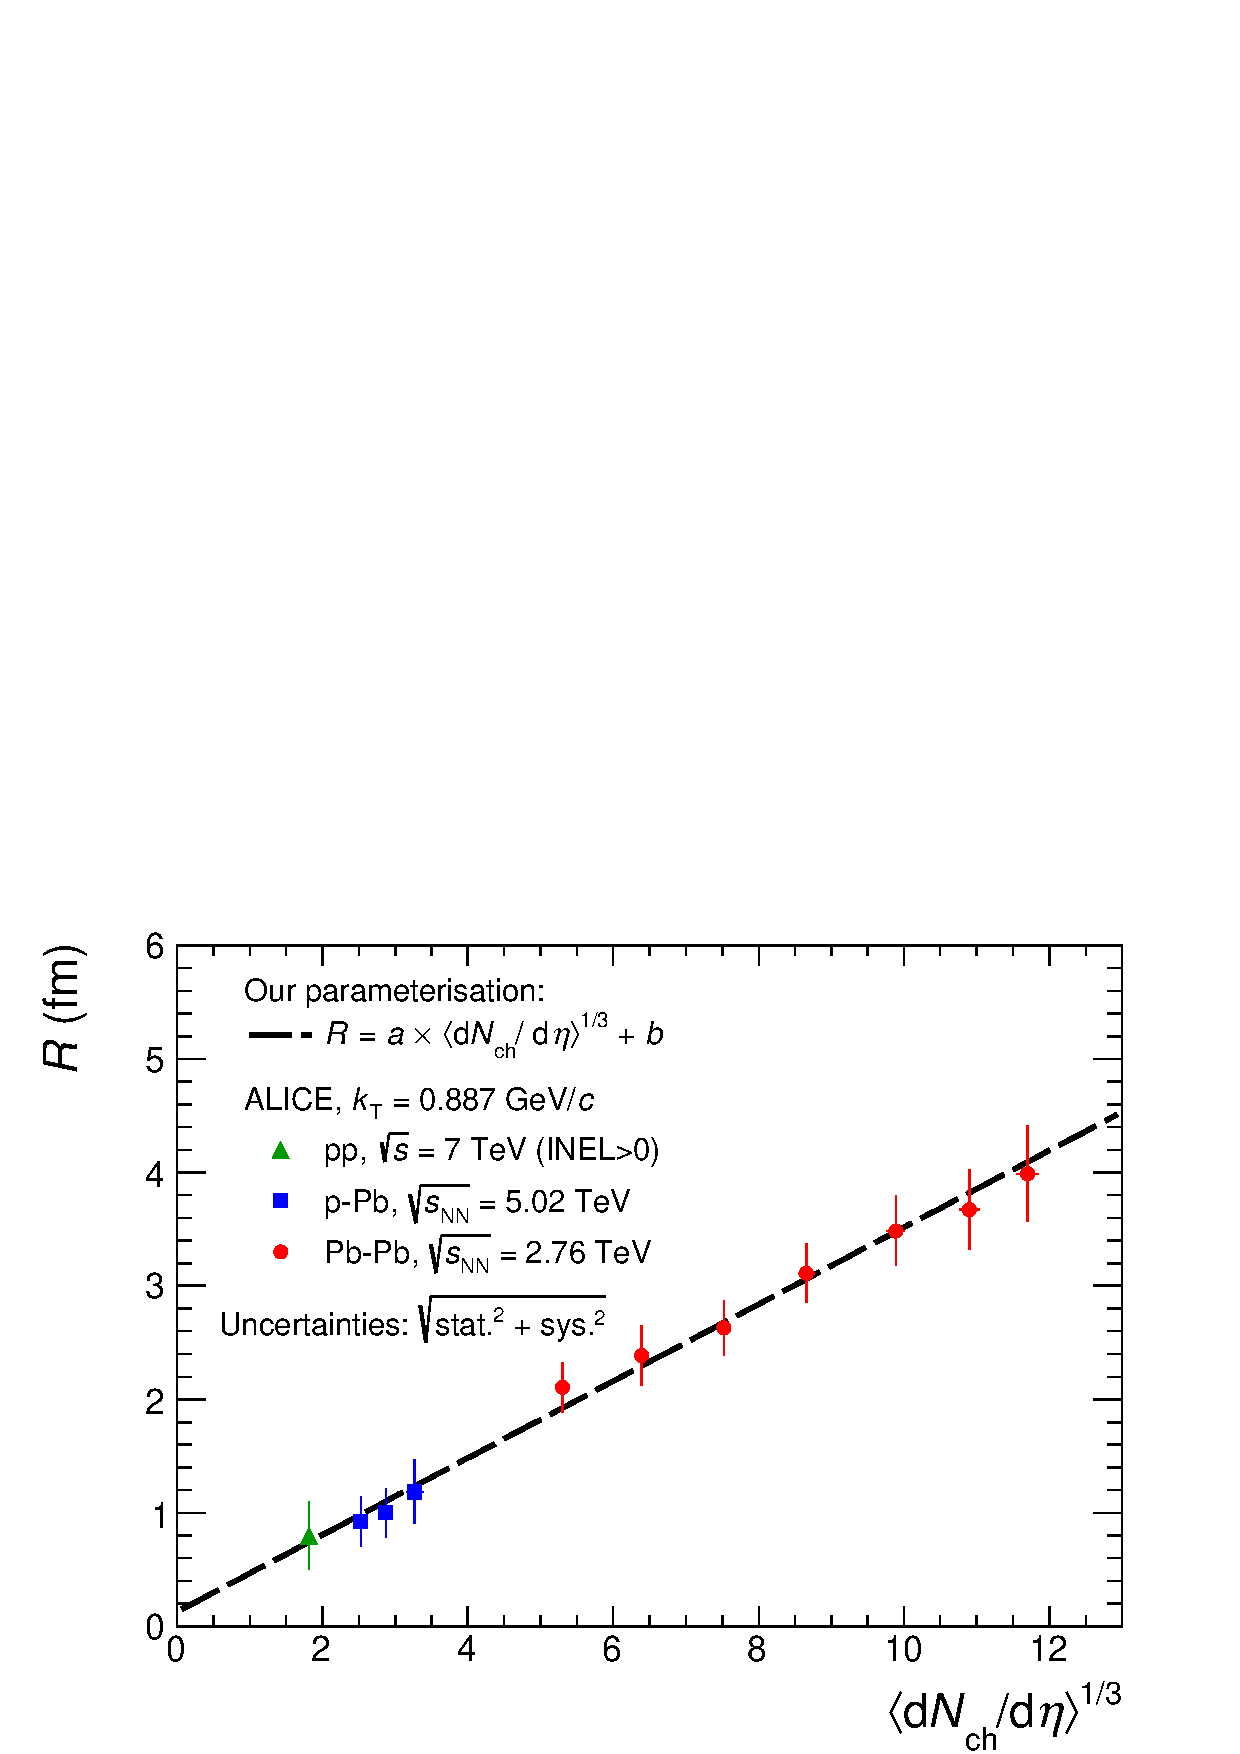
\includegraphics[width=\columnwidth]{../HbtRadiusParam.png}
\caption{Parameterisation A of the dependence of the source radius on multiplicity compared to HBT data from \cite{Adam:2015vna, Adam:2015pya, Abelev:2012sq}. The radius $R$ and the parameters $a$ and $b$ are in units of fm.}
\label{fig:radiiparam}
\end{center}
\end{figure}

\section{Statistical-thermal approach and blast-wave}\label{sec:thermal}

In the statistical-thermal approach \cite{Petran:2013dva,Wheaton:2004qb,Andronic:2005yp}, the yields (d$N$/d$y$) of light anti- and hyper-nuclei are very sensitive to $T_{chem}$ due to their large mass and approximately scale as d$N$/d$y \propto \exp(-m/T_{chem})$. 
At the LHC, the chemical potentials which ensure the conservation of baryon number, strangeness, and electric charge are negligible.
In contrast to coalescence, the statistical-thermal models provide only \pt-integrated yields. 
We use a blast-wave~\cite{Schnedermann:1993ws} parameterization to model the \pt-dependence, with parameters obtained from the simultaneous fit to pion, kaon and proton spectra measured in Pb--Pb collisions by ALICE~\cite{Abelev:2013vea}. 
The normalisation is fixed using the \pt-integrated deuteron-to-pion ratio and \hethree-to-pion ratio predicted by the GSI-Heidelberg model with $T_{chem} = 156$ MeV, multiplied by the measured pion yield~\cite{Abelev:2013vea}. 
This choice, as opposed to using the ratio to proton, is motivated by the fact that the measured proton yield is seen to be slightly overestimated by the thermal model~\cite{Abelev:2012wca}.
For hyper-triton, the normalisation is extracted from the statistical-thermal model prediction of the strangeness population factor $S_{3} = { _{\Lambda}^{3}\mathrm{H} / ^{3}{\mathrm{He}} \over \Lambda/p}$ multiplied by the measured $\Lambda/p$ ratio~\cite{Abelev:2013vea,Abelev:2013xaa} and \hethree~yield~\cite{ALICE:deuteronppPbPb2015}. 
With the resulting spectra, we calculate \bA~for a given \pt/$A$ and compare it with coalescence expectations. 
We use the corresponding \avdNdeta~in each class to estimate the system radius based on the parameterisation discussed in Sec.~\ref{SecSourceVolume}. 
In contrast to the coalescence approach, the object size does not enter in the formulation of the blast-wave model.
The thermal model on the other hand, implements eigenvolume corrections by fixing the object radius as an external parameter.
We refer to the literature for the extensive discussions on the validity of the eigenvolume correction for light (anti-)(hyper-)nuclei~\cite{Vovchenko:2016mwg} and the relation with the possible production as compact quark bags~\cite{Andronic:2017}.

\section{Constraining the source volume with data}\label{sec:radiiParamet}

Multiplicity-differential data on anti- and hyper-nuclei production at the LHC have been released by ALICE \cite{ALICE:nucleipp2017,ALICE:deuteronppPbPb2015,Acharya:2017dmc, Adam:2015yta}. 
To facilitate the comparison with multiplicity-dependent data given in the INEL$>$0 class, we have rescaled the inelastic pp collision data in \cite{ALICE:nucleipp2017} by the ratio of \avdNdeta~in these two event classes \cite{Adam:2015gka}.
In order to map \avdNdeta~to the source size we first used the parameterisation (labeled as ``A'') from the fit to the HBT data shown in Fig.~\ref{fig:radiiparam}. 
When comparing to data, we found a discrepancy between the coalescence volume from parameterisation A and the coalescence curve. 
In particular, the model would require a larger radius for a given value of \btwo~in Pb--Pb collisions.
In a second step we tuned the parameterisation (labeled as ``B'') such that the data points for (anti-)deuterons fall onto the coalescence prediction, finding the values $a = 0.473$ and $b = 0$ for Eq.~\ref{eq:radiusParameterisation}. 

With parameterisation B, we compare models to data, thus constraining the coalescence volume with the more differential (anti-)deuteron data and assuming that it is the same for all anti- and hyper-nuclei. 
The necessity of introducing a second parameterisation might suggest that the kinetic freeze-out volume relevant for coalescence is not given by the $m_{T}$-scaled pion HBT radius considered in parameterisation A, but by a slightly larger system as from parameterisation B.  

\section{Comparison with data}

In Fig.~\ref{fig:CompareThermalAndCoalescence}, the available data for (anti-)deuterons, \mbox{(anti-)}\hethree\ and (anti-)\hthreelambda~\cite{Adam:2015yta} are compared to coalescence and to the thermal model+blast wave predictions described in Sec.~\ref{sec:thermal}.
For the latter and for data, the radius parameterisation B is used, see Sec.~\ref{sec:radiiParamet}. 
For deuterons, both approaches lead to similar predictions and give a reasonable description of the experimental data for $R \gtrsim 1.6$ fm. 
For \hethree~the two models exhibit a qualitatively similar trend as a function of $R$, but they differ by a factor of about 1.5 to 2. The limited amount of data that is currently available is consistent with both models within 2$\sigma$ to 3$\sigma$, where $\sigma$ is the total uncertainty on the data. 
Both approaches show large differences (a factor 5 to 6 for central Pb--Pb collisions and a factor larger than 50 for small radii, $R < 2$ fm) for the \hthreelambda\ caused by the significantly larger size of \hthreelambda\ with respect to \hethree. 
The only data point available so far in Pb--Pb collisions is in agreement with the thermal model but not with coalescence. 
The difference between data and the coalescence model is about 6$\sigma$,
albeit the validity of our assumptions (\textit{in primis} the usage of a gaussian wave-function).
In \cite{Zhang:2018euf} it is argued that the difference between data and the coalescence model might be explained by a later formation through the coalescence of $\Lambda$s and deuterons. 
A possible difference attributable to the presence of excited states with $J=3/2$ of \hthreelambda, which would significantly enhance the phase space for its production, is not considered here as there is no evidence for its existence~\cite{Mart:1996ay}. 

Most importantly, Fig.~\ref{fig:CompareThermalAndCoalescence} shows that the difference between the two approaches increases with decreasing source volume, thus underlining the need for additional and more precise data as a function of multiplicity in order to distinguish between the two production scenarios. 
In the case of \hthreelambda~we have considered also a prediction from coalescence for a wider wave-function (dashed line in bottom right panel of Fig. \ref{fig:CompareThermalAndCoalescence}), which results in even lower production probabilities. This behaviour highlights the unique potential to constrain the wave-function of the particle under study at the moment of its production via precise measurements of the coalescence parameter as a function of the source volume. The curves presented here also explicitly allow for an estimate of the expected hyper-triton production in pp collisions, which is expected to be suppressed by about two orders of magnitude with respect to the production of \hethree, thus making this measurement a prime candidate for future experimental studies.
 \begin{figure}[ht]
	\begin{center}
		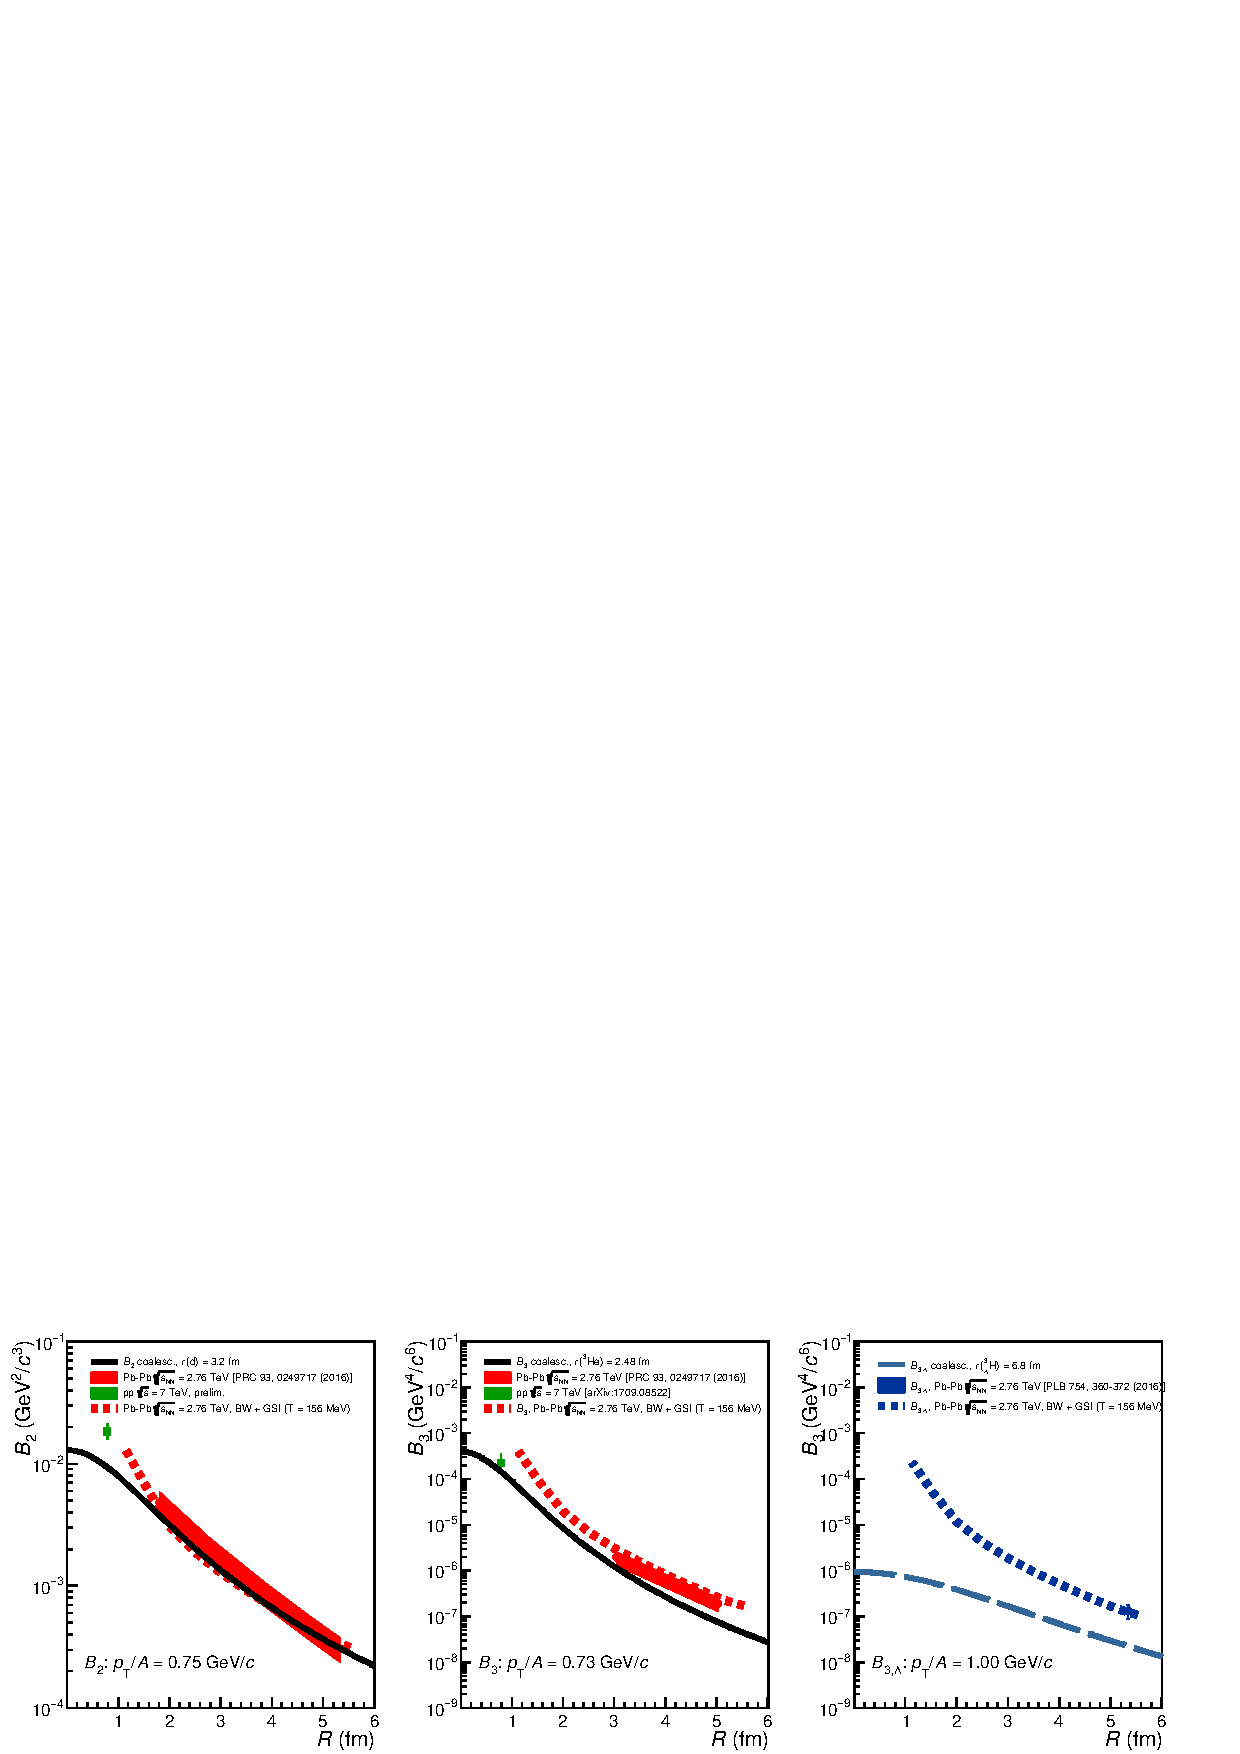
\includegraphics[width=.95\columnwidth]{../compareThermalAndCoalescence.png}
		\caption{Comparison of the coalescence parameters measured by ALICE (solid markers) for deuterons (upper panel), \hethree\ (middle panel) and \hthreelambda\ (lower panel) in pp \cite{ALICE:nucleipp2017} and Pb--Pb~\cite{ALICE:deuteronppPbPb2015, Adam:2015yta} collisions with the  thermal+blast-wave model expectations (dotted line) and the coalescence predictions (solid lines). Parameterisation B has been used to map \avdNdeta~into the radius $R$ of the source. The dashed line in the lower right panel corresponds to the coalescence prediction for the \hthreelambda\ with a larger radius.}
		\label{fig:CompareThermalAndCoalescence}
	\end{center}
\end{figure}

\section{Conclusions and outlook}
We summarise our main conclusions as follows:
\begin{enumerate}
	\item For the production of $A=2$ and $A=3$ (anti-)nuclei in heavy-ion collisions, the thermal and coalescence models give similar predictions for a source volume that is constrained by experimental data on d, $\bar{\mathrm{d}}$~production in central Pb--Pb collisions at the LHC.
	\item For the production of hyper-triton, the thermal and coalescence models give very different predictions as a function of source volume. In particular, the yield of hyper-triton appears to be suppressed by about two orders of magnitude in pp collisions with respect to the production of \hethree. The very limited amount of currently available data favours the thermal model prediction within our assumptions.
	\item Systematic measurements in pp, p--Pb, and Pb--Pb collisions at LHC energies have a unique potential to clarify the production mechanism and the nature of composite QCD objects. Ideally, such measurements are accompanied by systematic measurements of the HBT radii in the same multiplicity/centrality classes and collision systems.
\end{enumerate}

As our study is deliberately based on simplified assumptions that allow for a completely analytical treatment of the problem, future studies should be based on more realistic approximations (in particular the wave-function), which require numerical calculations. Moreover, it will be interesting to explore further the \pt~dependence of the observations made here.

In a follow-up publication, we plan to extend our study to predictions for the $A=4$ systems introduced in Tab.~\ref{tab:nucleusradii} and to more exotic QCD objects like the X(3872)~\cite{Esposito:2015fsa, Cho:2017dcy}. 
In fact, if the X(3872) corresponds to a loosely bound $\overline{D}^{*0}$--$D^{0}$ molecule, the rms of its wave-function can be as large as $4.9^{+13.4}_{-1.4}$~fm \cite{Artoisenet:2010uu}. Thus, its possible production via a coalescence mechanism in pp collisions would be subject to a similar suppression as the hyper-triton. 
The upcoming high-luminosity phase of the LHC (Run 3 $\&$ 4), where $A = 4$ hyper-nuclei and other rare composite objects will become experimentally accessible, will provide a unique opportunity for the final understanding of \mbox{(anti-)}(hyper-)nuclei production.
Setting a final word on the production mechanisms also has a broader application in astrophysics and dark-matter searches, by representing an essential input for the measurement of (anti-)nuclei in space with ongoing \cite{Alcaraz:2000ss, Poulin:2018wzu} and future \cite{AMS100, Aramaki:2015laa} experiments. 



\begin{acknowledgments}
We would like to thank Kfir Blum for inspiring this work. We thank U. Heinz for the useful discussions and the clarification on the equivalence of the Bertsch-Pratt and Yano-Koonin-Podgoretskii parameterisations of the HBT radii. We further acknowledge discussions with Benjamin Doenigus, in particular about the production of \hthreelambda\ in pp collisions, and with Eulogio Serradilla Rodriguez. In addition, we would like to thank Juergen Schukraft, Peter Braun-Munzinger, Maximiliano Puccio, Roman Lietava, Natasha Sharma and the colleagues from the ALICE Collaboration for their valuable input. 
\end{acknowledgments}

\bibliography{NucleiB2}
\end{document}
